The primary challenge in any text based modelling approach is the representation of data. A computer cannot comprehend words like humans, so it needs a numeric approach for text analysis. This leads to the idea of using ids to map words ~\parencite{nlpfundamentals}. For example, consider the sentence: “John went to the park.”. We can easily construct a basic dictionary for the words in this sentence and map them to a unique id as such: 

$\{"john" : 0, "went" : 1, "to" : 2, "the" : 3, "park" : 4\}$

\subsubsection{One-Hot Encoding}
This process could also occur for labels/categories that need to be numerically represented, such as colors or publications. However, there is a very obvious issue with this approach when using it on unordered data without obvious spatial relationships. This type of map tells the model that “park” is more important, or weighted more heavily, than “john”. If the model calculates averages, it will find the average of the words “went” and “the” to equal “to”. These types of relationships are obviously fraught and would cause major errors in the model’s effectiveness. To mitigate this problem, researchers developed the concept of one hot encoding, which essentially binarizes the process of mapping items to their numeric representations ~\parencite{harris_harris_2015}. A matrix is generated with dimensions length of items in entry X length of total dictionary for each example. Each row of the matrix has a single one and all other entries are zero to represent the single word. Using the above example, our sentence representation would become:

\[\begin{bmatrix}
1 & 0 & 0 & 0 & 0\\
0 & 1 & 0 & 0 & 0\\
0 & 0 & 1 & 0 & 0\\
0 & 0 & 0 & 1 & 0\\
0 & 0 & 0 & 0 & 1\\
\end{bmatrix}\]

Although this mitigates the earlier concerns, there are a variety of disadvantages to this approach. Firstly, the creation of such sparse matrices for each entry in the dataset, which can span millions of entries, is inefficient for storage purposes. It is also plagued by the “curse of dimensionality” as each category/word appends an entire dimension to the matrix. Finally, the adding of items to the dictionary would lead to changing the representations for all previous words. Aside from the structural issues, this approach lacks interpretability. As the items are fed into the model, the one-hot encoded matrix tells the user nothing about the relationship between words. It also breaks down any order of words, which is required for models such as \acrshort{bert}.

\subsubsection{Embedding Vectors}
These major problems with one-hot encoding led to the development of embeddings and vectorized representations of words in natural language processing. The fundamental premise of word embeddings is the concept that each word maps to a unique n-sized vector of a single dimension. Thus, words can be mapped to ids as they were above, and a separate mapping of ids to vectors can be utilized to convert each word into a corresponding mathematical representation. The embeddings are obviously not directly interpretable by humans, as they capture latent qualities of the word as the model is trained, however embeddings offer a significant advantage over one-hot encoding in their ability to offer comprehensible representations. Similar words will be found to be spatially contiguous. The relationship between words can also be calculated directly through cosine similarity, which is essentially the arccosine of the dot product of two vectors normalized by their magnitudes. The most famous example of this type of interpretability is the mathematical relationship \textbf{king - man + woman = queen} which can be graphically observed in Figure 1, produced by \textcite{king_man_woman_queen}: 

\begin{figure}[h]
\centering
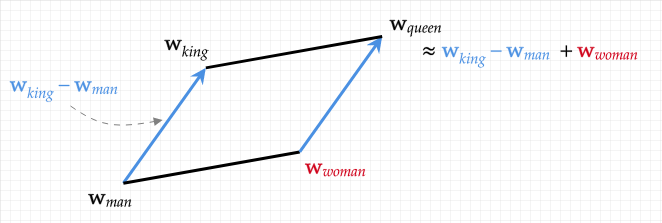
\includegraphics[width=0.8\textwidth]{fig/king-man-woman-queen.png}
\caption{Spatial representation of king - man + woman = queen}
\label{fig:king_man_woman_queen_pic}
\end{figure}

This then allows for each example in the dataset to be represented as a unidimensional list of word ids, which can then be mapped to their corresponding vectors when being processed by the model. The data storage advantages are obvious, as each entry becomes easily stored as a single dense list instead of the highly-sparse matrices generated by one-hot encoding. Thus, because of both the data-related and interpretability advantages offered by embeddings, they were utilized for both of the tested models.